\chapter{Grafos dirigidos}

En este capítulo veremos dos clases de grafos dirigidos:
\begin{itemize}
    \item \key{Grafos acíclicos}: No hay ciclos en el grafo, por lo que
          no existe un camino desde un nodo hacia sí mismo\footnote{Los
              grafos dirigidos acíclicos suelen llamarse DAGs, por
              \textit{directed acyclic graph}.}
    \item \key{Grafo sucesor}: El grado de salida de cada nodo es 1,
          por lo que cada nodo tiene un \emph{sucesor} único
\end{itemize}

Resulta que en los dos casos, podemos diseñar algoritmos eficientes
que están basados en las propiedades especiales de los grafos.

\section{Ordenamiento topológico}

\index{ordenamiento topológico}
\index{ciclo}

Un \key{ordenamiento topológico} es un ordenamiento de los nodos
de un grafo dirigido tal que si hay un camino desde un nodo $a$ a un
nodo $b$, entonces el nodo $a$ aparece antes que $b$ en el ordenamiento.
Por ejemplo, para el grafo

\begin{center}
    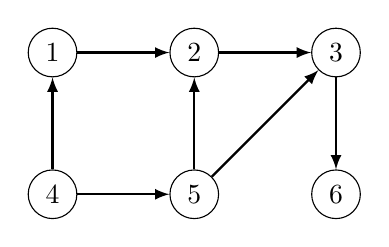
\begin{tikzpicture}[scale=0.9]
        \node[draw, circle] (1) at (1,5) {$1$};
        \node[draw, circle] (2) at (3,5) {$2$};
        \node[draw, circle] (3) at (5,5) {$3$};
        \node[draw, circle] (4) at (1,3) {$4$};
        \node[draw, circle] (5) at (3,3) {$5$};
        \node[draw, circle] (6) at (5,3) {$6$};

        \path[draw,thick,->,>=latex] (1) -- (2);
        \path[draw,thick,->,>=latex] (2) -- (3);
        \path[draw,thick,->,>=latex] (4) -- (1);
        \path[draw,thick,->,>=latex] (4) -- (5);
        \path[draw,thick,->,>=latex] (5) -- (2);
        \path[draw,thick,->,>=latex] (5) -- (3);
        \path[draw,thick,->,>=latex] (3) -- (6);
    \end{tikzpicture}
\end{center}

un ordenamiento topológico es $[4,1,5,2,3,6]$:
\begin{center}
    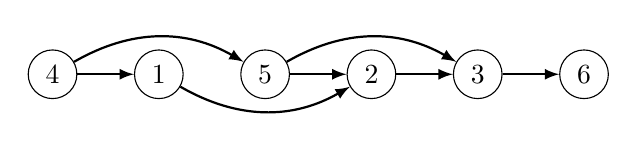
\begin{tikzpicture}[scale=0.9]
        \node[draw, circle] (1) at (-6,0) {$1$};
        \node[draw, circle] (2) at (-3,0) {$2$};
        \node[draw, circle] (3) at (-1.5,0) {$3$};
        \node[draw, circle] (4) at (-7.5,0) {$4$};
        \node[draw, circle] (5) at (-4.5,0) {$5$};
        \node[draw, circle] (6) at (-0,0) {$6$};

        \path[draw,thick,->,>=latex] (1) edge [bend right=30] (2);
        \path[draw,thick,->,>=latex] (2) -- (3);
        \path[draw,thick,->,>=latex] (4) -- (1);
        \path[draw,thick,->,>=latex] (4) edge [bend left=30] (5);
        \path[draw,thick,->,>=latex] (5) -- (2);
        \path[draw,thick,->,>=latex] (5) edge [bend left=30]  (3);
        \path[draw,thick,->,>=latex] (3) -- (6);
    \end{tikzpicture}
\end{center}

Un grafo acíclico siempre tiene un ordenamiento topológico.
Sin embargo, si el grafo contiene un ciclo, no es posible formar
un ordenamiento topológico, porque ningún nodo del ciclo podría
aparecer antes que los otros nodos del ciclo en el ordenamiento.
Resulta que la búsqueda en profundidad puede utilizarse para
revisar si el grafo dirigido contiene un ciclo y, si no es así,
para construir un ordenamiento topológico.

\subsubsection{Algoritmo}

La idea es recorrer los nodos del grafo y siempre comenzar
una búsqueda en profundidad en el nodo actual si todavía no ha sido
procesado. Durante las búsquedas, los nodos tienen tres posibles estados:

\begin{itemize}
    \item estado 0: el nodo no ha sido procesado (blanco)
    \item estado 1: el nodo está siendo procesado (gris claro)
    \item estado 2: el nodo ha sido procesado (gris oscuro)
\end{itemize}

Inicialmente, el estado de cada nodo es 0. Cuando una búsqueda
llega a un nodo por primera vez, su estado se vuelve 1. Finalmente,
una vez que todos los sucesores del nodo han sido procesados,
su estado se vuelve 2.

Si el grafo contiene un ciclo, nos daremos cuenta de esto
durante la búsqueda, porque tarde o temprano llegaremos a un
nodo cuyo estado es 1. En este caso, no es posible construir un
ordenamiento topológico.

Si el grafo no contiene ningún ciclo, podemos construir un ordenamiento
topológico agregando cada nodo a una lista cuando el estado del nodo
se vuelva 2. Esta lista, en orden inverso, es un ordenamiento topológico.

\subsubsection{Ejemplo 1}

En el grafo de ejemplo, el primer recorrido pasa del nodo 1 al nodo 6:
\begin{center}
    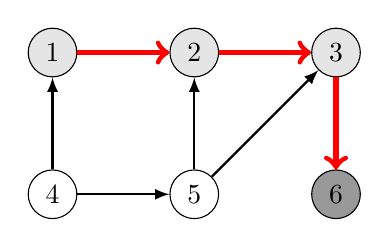
\begin{tikzpicture}[scale=0.9]
        \node[draw, circle,fill=gray!20] (1) at (1,5) {$1$};
        \node[draw, circle,fill=gray!20] (2) at (3,5) {$2$};
        \node[draw, circle,fill=gray!20] (3) at (5,5) {$3$};
        \node[draw, circle] (4) at (1,3) {$4$};
        \node[draw, circle] (5) at (3,3) {$5$};
        \node[draw, circle,fill=gray!80] (6) at (5,3) {$6$};

        \path[draw,thick,->,>=latex] (4) -- (1);
        \path[draw,thick,->,>=latex] (4) -- (5);
        \path[draw,thick,->,>=latex] (5) -- (2);
        \path[draw,thick,->,>=latex] (5) -- (3);
        %\path[draw,thick,->,>=latex] (3) -- (6);

        \path[draw=red,thick,->,line width=2pt] (1) -- (2);
        \path[draw=red,thick,->,line width=2pt] (2) -- (3);
        \path[draw=red,thick,->,line width=2pt] (3) -- (6);
    \end{tikzpicture}
\end{center}

Ahora el nodo 6 ha sido procesado, así que es añadido a la lista.
Luego, también los nodos 3, 2, y 1 son añadidos a la lista:
\begin{center}
    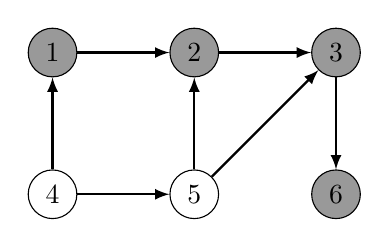
\begin{tikzpicture}[scale=0.9]
        \node[draw, circle,fill=gray!80] (1) at (1,5) {$1$};
        \node[draw, circle,fill=gray!80] (2) at (3,5) {$2$};
        \node[draw, circle,fill=gray!80] (3) at (5,5) {$3$};
        \node[draw, circle] (4) at (1,3) {$4$};
        \node[draw, circle] (5) at (3,3) {$5$};
        \node[draw, circle,fill=gray!80] (6) at (5,3) {$6$};

        \path[draw,thick,->,>=latex] (1) -- (2);
        \path[draw,thick,->,>=latex] (2) -- (3);
        \path[draw,thick,->,>=latex] (4) -- (1);
        \path[draw,thick,->,>=latex] (4) -- (5);
        \path[draw,thick,->,>=latex] (5) -- (2);
        \path[draw,thick,->,>=latex] (5) -- (3);
        \path[draw,thick,->,>=latex] (3) -- (6);
    \end{tikzpicture}
\end{center}

En este punto, la lista es $[6,3,2,1]$.
La búsqueda comienza en el nodo 4:

\begin{center}
    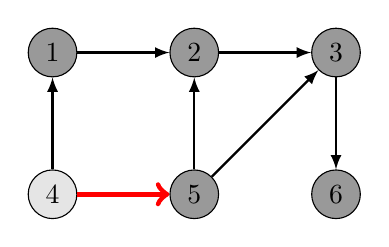
\begin{tikzpicture}[scale=0.9]
        \node[draw, circle,fill=gray!80] (1) at (1,5) {$1$};
        \node[draw, circle,fill=gray!80] (2) at (3,5) {$2$};
        \node[draw, circle,fill=gray!80] (3) at (5,5) {$3$};
        \node[draw, circle,fill=gray!20] (4) at (1,3) {$4$};
        \node[draw, circle,fill=gray!80] (5) at (3,3) {$5$};
        \node[draw, circle,fill=gray!80] (6) at (5,3) {$6$};

        \path[draw,thick,->,>=latex] (1) -- (2);
        \path[draw,thick,->,>=latex] (2) -- (3);
        \path[draw,thick,->,>=latex] (4) -- (1);
        %\path[draw,thick,->,>=latex] (4) -- (5);
        \path[draw,thick,->,>=latex] (5) -- (2);
        \path[draw,thick,->,>=latex] (5) -- (3);
        \path[draw,thick,->,>=latex] (3) -- (6);

        \path[draw=red,thick,->,line width=2pt] (4) -- (5);
    \end{tikzpicture}
\end{center}

Por ende, la lista final es $[6,3,2,1,5,4]$. Hemos procesado
todos los nodos, y encontramos un ordenamiento topológico; la
inversión $[4,5,1,2,3,6]$:

\begin{center}
    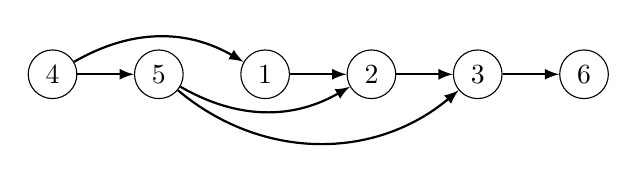
\begin{tikzpicture}[scale=0.9]
        \node[draw, circle] (1) at (3,0) {$1$};
        \node[draw, circle] (2) at (4.5,0) {$2$};
        \node[draw, circle] (3) at (6,0) {$3$};
        \node[draw, circle] (4) at (0,0) {$4$};
        \node[draw, circle] (5) at (1.5,0) {$5$};
        \node[draw, circle] (6) at (7.5,0) {$6$};

        \path[draw,thick,->,>=latex] (1) -- (2);
        \path[draw,thick,->,>=latex] (2) -- (3);
        \path[draw,thick,->,>=latex] (4) edge [bend left=30] (1);
        \path[draw,thick,->,>=latex] (4) -- (5);
        \path[draw,thick,->,>=latex] (5) edge [bend right=30] (2);
        \path[draw,thick,->,>=latex] (5) edge [bend right=40] (3);
        \path[draw,thick,->,>=latex] (3) -- (6);
    \end{tikzpicture}
\end{center}

Ten en cuenta que un ordenamiento topológico no es único, por lo que
pueden existir varios dado un solo grafo.

\subsubsection{Ejemplo 2}

Ahora, veamos un grafo cuyo ordenamiento topológico no existe,
ya que el grafo contiene un ciclo:

\begin{center}
    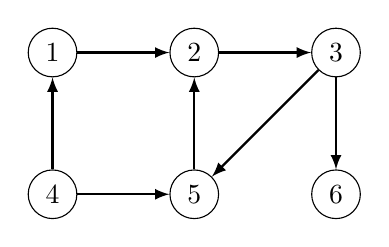
\begin{tikzpicture}[scale=0.9]
        \node[draw, circle] (1) at (1,5) {$1$};
        \node[draw, circle] (2) at (3,5) {$2$};
        \node[draw, circle] (3) at (5,5) {$3$};
        \node[draw, circle] (4) at (1,3) {$4$};
        \node[draw, circle] (5) at (3,3) {$5$};
        \node[draw, circle] (6) at (5,3) {$6$};

        \path[draw,thick,->,>=latex] (1) -- (2);
        \path[draw,thick,->,>=latex] (2) -- (3);
        \path[draw,thick,->,>=latex] (4) -- (1);
        \path[draw,thick,->,>=latex] (4) -- (5);
        \path[draw,thick,->,>=latex] (5) -- (2);
        \path[draw,thick,->,>=latex] (3) -- (5);
        \path[draw,thick,->,>=latex] (3) -- (6);
    \end{tikzpicture}
\end{center}

La búsqueda procede de la siguiente manera:
\begin{center}
    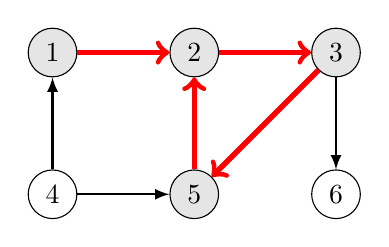
\begin{tikzpicture}[scale=0.9]
        \node[draw, circle,fill=gray!20] (1) at (1,5) {$1$};
        \node[draw, circle,fill=gray!20] (2) at (3,5) {$2$};
        \node[draw, circle,fill=gray!20] (3) at (5,5) {$3$};
        \node[draw, circle] (4) at (1,3) {$4$};
        \node[draw, circle,fill=gray!20] (5) at (3,3) {$5$};
        \node[draw, circle] (6) at (5,3) {$6$};

        \path[draw,thick,->,>=latex] (4) -- (1);
        \path[draw,thick,->,>=latex] (4) -- (5);
        \path[draw,thick,->,>=latex] (3) -- (6);

        \path[draw=red,thick,->,line width=2pt] (1) -- (2);
        \path[draw=red,thick,->,line width=2pt] (2) -- (3);
        \path[draw=red,thick,->,line width=2pt] (3) -- (5);
        \path[draw=red,thick,->,line width=2pt] (5) -- (2);
    \end{tikzpicture}
\end{center}

La búsqueda llega al nodo 2, cuyo estado es 1, lo que significa que
el grafo contiene un ciclo. En este ejemplo, existe el ciclo
$2 \rightarrow 3 \rightarrow 5 \rightarrow 2$.

\section{Programación dinámica}

Si un grafo dirigido es acíclico, podemos aplicarle programación
dinámica. Por ejemplo, podemos resolver eficientemente los siguientes
problemas relacionados a caminos entre un nodo inicial y un nodo final:

\begin{itemize}
    \item ¿cuántos caminos diferentes existen?
    \item ¿cuál es el camino más corto/largo?
    \item ¿cuál es el número mínimo/máximo de aristas en un camino?
    \item ¿cuáles nodos definitivamente aparecen en cualquier camino?
\end{itemize}

\subsubsection{Contar el número de caminos}

Como ejemplo, calculemos el número de caminos desde el nodo 1
al nodo 6 en el siguiente grafo:
\begin{center}
    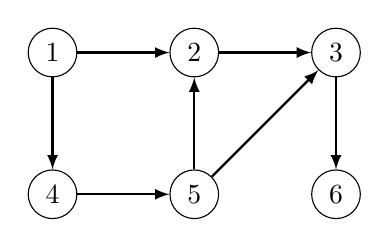
\begin{tikzpicture}[scale=0.9]
        \node[draw, circle] (1) at (1,5) {$1$};
        \node[draw, circle] (2) at (3,5) {$2$};
        \node[draw, circle] (3) at (5,5) {$3$};
        \node[draw, circle] (4) at (1,3) {$4$};
        \node[draw, circle] (5) at (3,3) {$5$};
        \node[draw, circle] (6) at (5,3) {$6$};

        \path[draw,thick,->,>=latex] (1) -- (2);
        \path[draw,thick,->,>=latex] (2) -- (3);
        \path[draw,thick,->,>=latex] (1) -- (4);
        \path[draw,thick,->,>=latex] (4) -- (5);
        \path[draw,thick,->,>=latex] (5) -- (2);
        \path[draw,thick,->,>=latex] (5) -- (3);
        \path[draw,thick,->,>=latex] (3) -- (6);
    \end{tikzpicture}
\end{center}

Hay un total de tres caminos:
\begin{itemize}
    \item $1 \rightarrow 2 \rightarrow 3 \rightarrow 6$
    \item $1 \rightarrow 4 \rightarrow 5 \rightarrow 2 \rightarrow 3 \rightarrow 6$
    \item $1 \rightarrow 4 \rightarrow 5 \rightarrow 3 \rightarrow 6$
\end{itemize}

Definamos $\texttt{caminos}(x)$ como el número de caminos desde el
nodo 1 al nodo $x$. Como caso base, $\texttt{caminos}(1)=1$. Entonces,
para calcular otros valores de $\texttt{caminos}(x)$, podemos utilizar
la recursión

\[\texttt{caminos}(x) = \texttt{caminos}(a_1)+\texttt{caminos}(a_2)+\cdots+\texttt{caminos}(a_k)\]

donde $a_1,a_2,\ldots,a_k$ son los nodos desde los cuales existe una
arista hacia el nodo $x$. Debido a que el grafo es acíclico, los valores
de $\texttt{caminos}(x)$ pueden ser calculados en el orden de un
ordenamiento topológico. Un ordenamiento topológico para el grafo de
arriba es el siguiente:

\begin{center}
    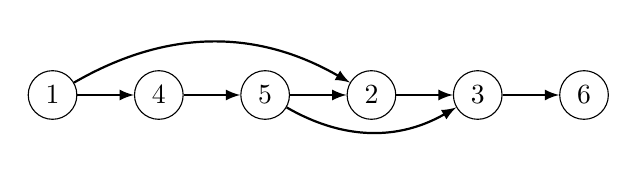
\begin{tikzpicture}[scale=0.9]
        \node[draw, circle] (1) at (0,0) {$1$};
        \node[draw, circle] (2) at (4.5,0) {$2$};
        \node[draw, circle] (3) at (6,0) {$3$};
        \node[draw, circle] (4) at (1.5,0) {$4$};
        \node[draw, circle] (5) at (3,0) {$5$};
        \node[draw, circle] (6) at (7.5,0) {$6$};

        \path[draw,thick,->,>=latex] (1) edge [bend left=30] (2);
        \path[draw,thick,->,>=latex] (2) -- (3);
        \path[draw,thick,->,>=latex] (1) -- (4);
        \path[draw,thick,->,>=latex] (4) -- (5);
        \path[draw,thick,->,>=latex] (5) -- (2);
        \path[draw,thick,->,>=latex] (5) edge [bend right=30] (3);
        \path[draw,thick,->,>=latex] (3) -- (6);
    \end{tikzpicture}
\end{center}

Por lo tanto, los números de caminos son los siguientes:
\begin{center}
    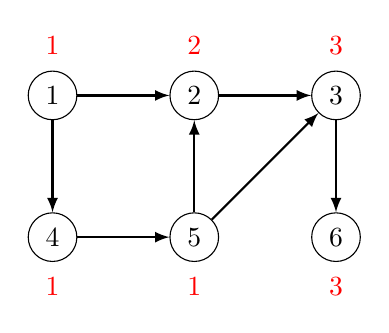
\begin{tikzpicture}[scale=0.9]
        \node[draw, circle] (1) at (1,5) {$1$};
        \node[draw, circle] (2) at (3,5) {$2$};
        \node[draw, circle] (3) at (5,5) {$3$};
        \node[draw, circle] (4) at (1,3) {$4$};
        \node[draw, circle] (5) at (3,3) {$5$};
        \node[draw, circle] (6) at (5,3) {$6$};

        \path[draw,thick,->,>=latex] (1) -- (2);
        \path[draw,thick,->,>=latex] (2) -- (3);
        \path[draw,thick,->,>=latex] (1) -- (4);
        \path[draw,thick,->,>=latex] (4) -- (5);
        \path[draw,thick,->,>=latex] (5) -- (2);
        \path[draw,thick,->,>=latex] (5) -- (3);
        \path[draw,thick,->,>=latex] (3) -- (6);

        \node[color=red] at (1,2.3) {$1$};
        \node[color=red] at (3,2.3) {$1$};
        \node[color=red] at (5,2.3) {$3$};
        \node[color=red] at (1,5.7) {$1$};
        \node[color=red] at (3,5.7) {$2$};
        \node[color=red] at (5,5.7) {$3$};
    \end{tikzpicture}
\end{center}

Por ejemplo, para calcular el valor de $\texttt{caminos}(3)$,
podemos utilizar la fórmula $\texttt{caminos}(2)+\texttt{caminos}(5)$,
porque existen aristas desde los nodos 2 y 5 al nodo 3.
Como $\texttt{caminos}(2)=2$ y $\texttt{caminos}(5)=1$, concluimos
que $\texttt{caminos}(3)=3$.

\subsubsection{Extendiendo el algoritmo de Dijkstra}

\index{algoritmo de Dijkstra}

Un subproducto del algoritmo de Dijkstra es un grafo acíclico dirigido
que indica, para cada nodo del grafo original, las formas posibles
de alcanzar el nodo utilizando el camino más corto desde el nodo inicial.
Podemos aplicar programación dinámica a ese grafo. Por ejemplo,
en el grafo

\begin{center}
    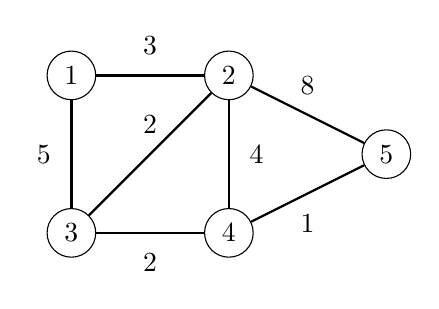
\begin{tikzpicture}
        \node[draw, circle] (1) at (0,0) {$1$};
        \node[draw, circle] (2) at (2,0) {$2$};
        \node[draw, circle] (3) at (0,-2) {$3$};
        \node[draw, circle] (4) at (2,-2) {$4$};
        \node[draw, circle] (5) at (4,-1) {$5$};

        \path[draw,thick,-] (1) -- node[font=\small,label=above:3] {} (2);
        \path[draw,thick,-] (1) -- node[font=\small,label=left:5] {} (3);
        \path[draw,thick,-] (2) -- node[font=\small,label=right:4] {} (4);
        \path[draw,thick,-] (2) -- node[font=\small,label=above:8] {} (5);
        \path[draw,thick,-] (3) -- node[font=\small,label=below:2] {} (4);
        \path[draw,thick,-] (4) -- node[font=\small,label=below:1] {} (5);
        \path[draw,thick,-] (2) -- node[font=\small,label=above:2] {} (3);
    \end{tikzpicture}
\end{center}

los caminos mínimos desde el nodo 1 pueden utilizar las siguientes aristas:
\begin{center}
    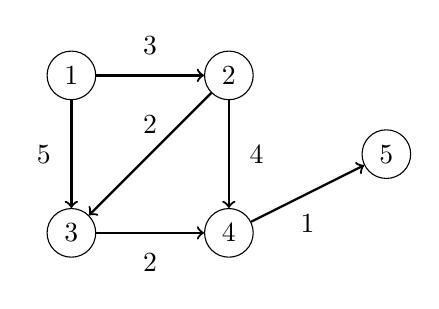
\begin{tikzpicture}
        \node[draw, circle] (1) at (0,0) {$1$};
        \node[draw, circle] (2) at (2,0) {$2$};
        \node[draw, circle] (3) at (0,-2) {$3$};
        \node[draw, circle] (4) at (2,-2) {$4$};
        \node[draw, circle] (5) at (4,-1) {$5$};

        \path[draw,thick,->] (1) -- node[font=\small,label=above:3] {} (2);
        \path[draw,thick,->] (1) -- node[font=\small,label=left:5] {} (3);
        \path[draw,thick,->] (2) -- node[font=\small,label=right:4] {} (4);
        \path[draw,thick,->] (3) -- node[font=\small,label=below:2] {} (4);
        \path[draw,thick,->] (4) -- node[font=\small,label=below:1] {} (5);
        \path[draw,thick,->] (2) -- node[font=\small,label=above:2] {} (3);
    \end{tikzpicture}
\end{center}

Ahora podemos, por ejemplo, calcular el número de caminos mínimos
entre del nodo 1 al nodo 5 utilizando la programación dinámica:
\begin{center}
    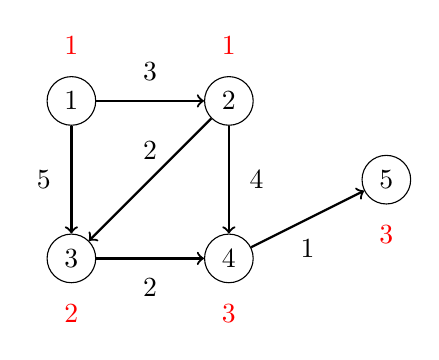
\begin{tikzpicture}
        \node[draw, circle] (1) at (0,0) {$1$};
        \node[draw, circle] (2) at (2,0) {$2$};
        \node[draw, circle] (3) at (0,-2) {$3$};
        \node[draw, circle] (4) at (2,-2) {$4$};
        \node[draw, circle] (5) at (4,-1) {$5$};

        \path[draw,thick,->] (1) -- node[font=\small,label=above:3] {} (2);
        \path[draw,thick,->] (1) -- node[font=\small,label=left:5] {} (3);
        \path[draw,thick,->] (2) -- node[font=\small,label=right:4] {} (4);
        \path[draw,thick,->] (3) -- node[font=\small,label=below:2] {} (4);
        \path[draw,thick,->] (4) -- node[font=\small,label=below:1] {} (5);
        \path[draw,thick,->] (2) -- node[font=\small,label=above:2] {} (3);

        \node[color=red] at (0,0.7) {$1$};
        \node[color=red] at (2,0.7) {$1$};
        \node[color=red] at (0,-2.7) {$2$};
        \node[color=red] at (2,-2.7) {$3$};
        \node[color=red] at (4,-1.7) {$3$};
    \end{tikzpicture}
\end{center}

\subsubsection{Representar problemas con grafos}

De hecho, cualquier problema de programación dinámica puede ser
representado como un grafo acíclico dirigido. En tal grafo, cada
nodo corresponde a un estado de programación dinámica, y las aristas
indican sus interdependencias.

Como ejemplo, considera el problema de formar una suma de dinero $n$
utilizando las monedas $\{m_1,m_2,\ldots,m_k\}$. En este problema,
podemos construir un grafo en el que cada nodo corresponde a una suma
de dinero, y las aristas muestran cómo las monedas pueden elegirse.
Por ejemplo, para las monedas $\{1,3,4\}$ y $n=6$, el gráfico se ve así:
\begin{center}
    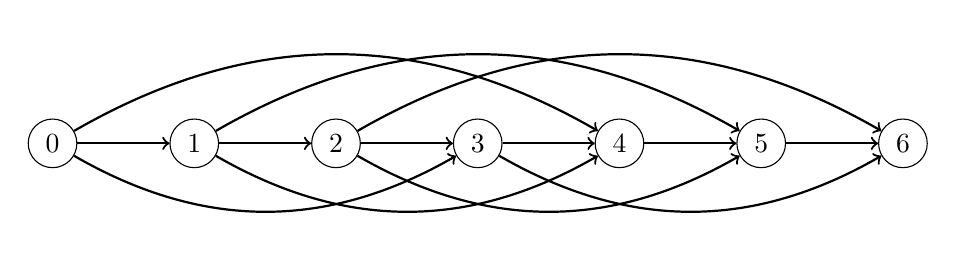
\begin{tikzpicture}[scale=0.9]
        \node[draw, circle] (0) at (0,0) {$0$};
        \node[draw, circle] (1) at (2,0) {$1$};
        \node[draw, circle] (2) at (4,0) {$2$};
        \node[draw, circle] (3) at (6,0) {$3$};
        \node[draw, circle] (4) at (8,0) {$4$};
        \node[draw, circle] (5) at (10,0) {$5$};
        \node[draw, circle] (6) at (12,0) {$6$};

        \path[draw,thick,->] (0) -- (1);
        \path[draw,thick,->] (1) -- (2);
        \path[draw,thick,->] (2) -- (3);
        \path[draw,thick,->] (3) -- (4);
        \path[draw,thick,->] (4) -- (5);
        \path[draw,thick,->] (5) -- (6);

        \path[draw,thick,->] (0) edge [bend right=30] (3);
        \path[draw,thick,->] (1) edge [bend right=30] (4);
        \path[draw,thick,->] (2) edge [bend right=30] (5);
        \path[draw,thick,->] (3) edge [bend right=30] (6);

        \path[draw,thick,->] (0) edge [bend left=30] (4);
        \path[draw,thick,->] (1) edge [bend left=30] (5);
        \path[draw,thick,->] (2) edge [bend left=30] (6);
    \end{tikzpicture}
\end{center}

Utilizando esta representación, el camino mínimo de nodo 0 al nodo $n$
corresponde a una solución con el mínimo número de monedas, y el
número total de caminos del nodo 0 al nodo $n$ equivale al número
total de soluciones.

\section{Grafos sucesores}

\index{grafo sucesor}
\index{grafo funcional}

Por el resto del capítulo, veremos \key{grafos sucesores}. En estos
grafos, el grado de salida de cada nodo es 1, o sea, exactamente una
arista comienza en cada nodo. Un grafo sucesor consiste de uno o más
componentes, cada uno de los cuales contiene un ciclo y algunos caminos
que conducen a él.

Los grafos sucesores son a veces llamados \key{grafos funcionales},
porque cualquier grafo sucesor corresponde a una función que define
aristas del grafo. El parámetro de la función es un nodo del grafo,
y su retorno es el sucesor de ese nodo.

Por ejemplo, la función
\begin{center}
    \begin{tabular}{r|rrrrrrrrr}
        $x$               & 1 & 2 & 3 & 4 & 5 & 6 & 7 & 8 & 9 \\
        \hline
        $\texttt{suc}(x)$ & 3 & 5 & 7 & 6 & 2 & 2 & 1 & 6 & 3 \\
    \end{tabular}
\end{center}

define el siguiente grafo:
\begin{center}
    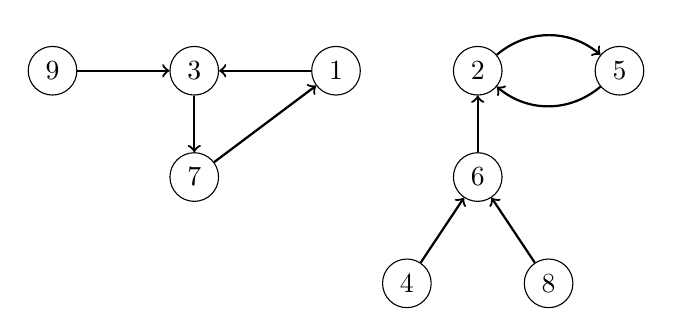
\begin{tikzpicture}[scale=0.9]
        \node[draw, circle] (1) at (0,0) {$1$};
        \node[draw, circle] (2) at (2,0) {$2$};
        \node[draw, circle] (3) at (-2,0) {$3$};
        \node[draw, circle] (4) at (1,-3) {$4$};
        \node[draw, circle] (5) at (4,0) {$5$};
        \node[draw, circle] (6) at (2,-1.5) {$6$};
        \node[draw, circle] (7) at (-2,-1.5) {$7$};
        \node[draw, circle] (8) at (3,-3) {$8$};
        \node[draw, circle] (9) at (-4,0) {$9$};

        \path[draw,thick,->] (1) -- (3);
        \path[draw,thick,->] (2)  edge [bend left=40] (5);
        \path[draw,thick,->] (3) -- (7);
        \path[draw,thick,->] (4) -- (6);
        \path[draw,thick,->] (5)  edge [bend left=40] (2);
        \path[draw,thick,->] (6) -- (2);
        \path[draw,thick,->] (7) -- (1);
        \path[draw,thick,->] (8) -- (6);
        \path[draw,thick,->] (9) -- (3);
    \end{tikzpicture}
\end{center}

Debido a que cada nodo de un grafo sucesor tiene un sucesor único,
también podemos definir una función $\texttt{suc}(x,k)$ que devuelve
el nodo que alcanzaremos si empezamos en el nodo $x$ y caminamos $k$
pasos para adelante. Por ejemplo, en el grafo anterior
$\texttt{suc}(4,6)=2$, porque si damos 6 pasos desde el nodo 4
alcanzaremos el nodo 2:

\begin{center}
    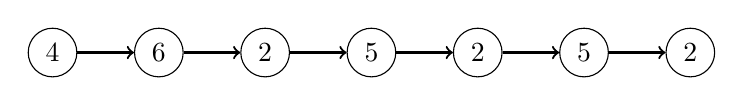
\begin{tikzpicture}[scale=0.9]
        \node[draw, circle] (1) at (0,0) {$4$};
        \node[draw, circle] (2) at (1.5,0) {$6$};
        \node[draw, circle] (3) at (3,0) {$2$};
        \node[draw, circle] (4) at (4.5,0) {$5$};
        \node[draw, circle] (5) at (6,0) {$2$};
        \node[draw, circle] (6) at (7.5,0) {$5$};
        \node[draw, circle] (7) at (9,0) {$2$};

        \path[draw,thick,->] (1) -- (2);
        \path[draw,thick,->] (2) -- (3);
        \path[draw,thick,->] (3) -- (4);
        \path[draw,thick,->] (4) -- (5);
        \path[draw,thick,->] (5) -- (6);
        \path[draw,thick,->] (6) -- (7);
    \end{tikzpicture}
\end{center}

Una forma sencilla de calcular el valor de $\texttt{suc}(x,k)$ es
comenzar en el nodo $x$ y dar $k$ pasos, que tarda $O(k)$.
De todas formas, usando preprocesamiento, cualquier valor de
$\texttt{suc}(x,k)$ puede calcularse en solo $O(\log k)$.

La idea es precalcular todo valor de $\texttt{suc}(x,k)$ dado que
$k$ sea una potencia de 2 y como mucho $u$, donde $u$ es el número
máximo de pasos que vamos a dar. Esto puede hacerse eficientemente
utilizando la siguiente recursión:

\begin{equation*}
    \texttt{suc}(x,k) = \begin{cases}
        \texttt{suc}(x)                                       & k = 1 \\
        \texttt{suc}(\texttt{suc}(x,\frac{k}{2}),\frac{k}{2}) & k > 1 \\
    \end{cases}
\end{equation*}

Precalcular los valores toma $O(n \log u)$, porque se calculan
$O(\log u)$ valores por cada nodo. En el grafo de arriba, los primeros
valores se ven así:

\begin{center}
    \begin{tabular}{r|rrrrrrrrr}
        $x$                 & 1 & 2 & 3 & 4 & 5 & 6 & 7 & 8 & 9 \\
        \hline
        $\texttt{suc}(x,1)$ & 3 & 5 & 7 & 6 & 2 & 2 & 1 & 6 & 3 \\
        $\texttt{suc}(x,2)$ & 7 & 2 & 1 & 2 & 5 & 5 & 3 & 2 & 7 \\
        $\texttt{suc}(x,4)$ & 3 & 2 & 7 & 2 & 5 & 5 & 1 & 2 & 3 \\
        $\texttt{suc}(x,8)$ & 7 & 2 & 1 & 2 & 5 & 5 & 3 & 2 & 7 \\
        $\cdots$                                                \\
    \end{tabular}
\end{center}

Ahora, cualquier valor de $\texttt{suc}(x,k)$ puede calcularse si
representamos $k$ como una suma de potencias de 2. Por ejemplo, si
queremos calcular el valor de $\texttt{suc}(x,11)$, primero formamos
la representación $11=8+2+1$. Utilizando esto,
\[\texttt{suc}(x,11)=\texttt{suc}(\texttt{suc}(\texttt{suc}(x,8),2),1).\]
Por ejemplo, en el grafo de arriba
\[\texttt{suc}(4,11)=\texttt{suc}(\texttt{suc}(\texttt{suc}(4,8),2),1)=5.\]

Tal representación siempre consiste de $O(\log k)$ partes,
así que calcular un valor de $\texttt{suc}(x,k)$ tarda $O(\log k)$.

\section{Detección de ciclos}

\index{ciclo}
\index{detección de ciclos}

Considera un grafo sucesor que solo contenga un camino que termina
en un ciclo. Podemos preguntar las siguientes preguntas: si comenzamos
nuestro recorrido en el nodo inicial, ¿cuál es el primer nodo en el ciclo
y cuántos nodos contiene?

Por ejemplo, en el grafo
\begin{center}
    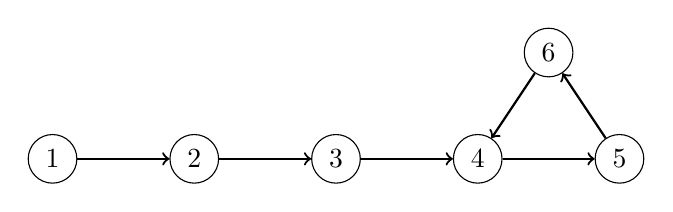
\begin{tikzpicture}[scale=0.9]
        \node[draw, circle] (5) at (0,0) {$5$};
        \node[draw, circle] (4) at (-2,0) {$4$};
        \node[draw, circle] (6) at (-1,1.5) {$6$};
        \node[draw, circle] (3) at (-4,0) {$3$};
        \node[draw, circle] (2) at (-6,0) {$2$};
        \node[draw, circle] (1) at (-8,0) {$1$};

        \path[draw,thick,->] (1) -- (2);
        \path[draw,thick,->] (2) -- (3);
        \path[draw,thick,->] (3) -- (4);
        \path[draw,thick,->] (4) -- (5);
        \path[draw,thick,->] (5) -- (6);
        \path[draw,thick,->] (6) -- (4);
    \end{tikzpicture}
\end{center}

comenzamos el recorrido en el nodo 1, el primer nodo que pertenece
al ciclo es el nodo 4, y el ciclo consiste en tres nodos (4, 5, y 6).

Una simple forma de detectar el ciclo es recorrer el grafo y mantener
un registro de todos los nodos que se han visitado. Una vez que un nodo
es visitado por segunda vez, podemos concluir que este es el primer nodo
en el ciclo. Este método funciona en $O(n)$ y también usa $O(n)$ de memoria.

No obstante, hay mejores algoritmos para la detección de ciclos. La
complejidad temporal de estos algoritmos sigue siendo $O(n)$, pero solo
usan $O(1)$ de memoria. Esta es una importante mejora si $n$ es muy grande.
Ahora veremos el algoritmo de Floyd que logra estas propiedades.

\subsubsection{Algoritmo de Floyd}

\index{algoritmo de Floyd}

El \key{algoritmo de Floyd}\footnote{La idea de este algoritmo es
    mencionada en \cite{knu982} y atribuida a R. W. Floyd; sin embargo,
    se desconoce si Floyd verdaderamente descubrió el algoritmo.}
recorre el grafo utilizando dos punteros $a$ y $b$. Los dos comienzan
en el nodo inicial $x$ y, en cada turno, el puntero $a$ camina un paso
y el puntero $b$ camina dos pasos. El proceso continúa hasta que los
dos punteros se encuentren:

\begin{lstlisting}
a = suc(x);
b = suc(suc(x));
while (a != b) {
    a = suc(a);
    b = suc(suc(b));
}
\end{lstlisting}

En este punto, el puntero $a$ ha caminado $k$ pasos y el puntero $b$
ha caminado $2k$ pasos, así que la longitud del ciclo es un divisor de $k$.
Por ende, el primer nodo que pertenece al ciclo puede encontrarse
moviendo el puntero $a$ al nodo $x$ y avanzando los punteros paso por
paso hasta que vuelvan a encontrarse.
\begin{lstlisting}
a = x;
while (a != b) {
    a = suc(a);
    b = suc(b);
}
primero = a;
\end{lstlisting}

Luego de esto, la longitud del ciclo puede calcularse de
la siguiente manera:
\begin{lstlisting}
b = suc(a);
longitud = 1;
while (a != b) {
    b = suc(b);
    longitud++;
}
\end{lstlisting}
